\documentclass[11pt,a4paper]{article}
\usepackage[utf8]{inputenc}
\usepackage{amsmath,amsfonts,amssymb}
\usepackage{graphicx}
\usepackage{geometry}
\geometry{margin=1in}
\usepackage{booktabs}
\usepackage{hyperref}
\usepackage{float}

\title{\textbf{EE3621: Digital Signal Processing} \\ \Large Lecture 4: Frequency Response, Magnitude/Phase \& Group Delay of LTI Systems \\ \large (III B.Tech EEE)}
\author{Lecture Notes (40-Minute Plan)}
\date{}

\usepackage{xcolor}
\definecolor{darkbg}{HTML}{0d121f}
\definecolor{lighttext}{HTML}{e2e8f0}
\definecolor{primary}{HTML}{8b5cf6}
\definecolor{secondary}{HTML}{0dd5c5}

\pagecolor{darkbg}
\color{lighttext}

\hypersetup{
    colorlinks=true,
    linkcolor=secondary,
    urlcolor=secondary
}

\begin{document}

\maketitle

\section{Lecture Plan \& Objectives (40 Minutes Breakdown)}
\begin{itemize}
    \item \textbf{00:00 -- 08:00 (8 mins):} LTI Eigenfunctions: Why complex exponentials are unique. Derivation of $H(e^{j\omega})$.
    \item \textbf{08:00 -- 15:00 (7 mins):} Magnitude \& Phase responses, Rectangular vs. Polar forms.
    \item \textbf{15:00 -- 25:00 (10 mins):} Phase Delay vs. Group Delay. Narrowband input derivation (Carrier vs. Envelope delay).
    \item \textbf{25:00 -- 35:00 (10 mins):} First-order IIR Filter Example: Detailed algebraic derivation of Group Delay.
    \item \textbf{35:00 -- 40:00 (5 mins):} Checkpoints \& Concept Recap.
\end{itemize}

\noindent\rule{\textwidth}{0.5pt}

\section{Eigenfunctions \& The Frequency Response}
Complex exponentials $e^{j\omega n}$ are eigenfunctions of linear time-invariant systems.
Let the input be $x[n] = e^{j\omega n}$ for $-\infty < n < \infty$. The output $y[n]$ is:
\begin{equation}
y[n] = \sum_{k=-\infty}^{\infty} h[k] x[n-k] = \sum_{k=-\infty}^{\infty} h[k] e^{j\omega(n-k)} = e^{j\omega n} \sum_{k=-\infty}^{\infty} h[k] e^{-j\omega k}
\end{equation}
We define the complex scaling factor (eigenvalue) as the frequency response $H(e^{j\omega})$:
\begin{equation}
y[n] = H(e^{j\omega}) e^{j\omega n}
\end{equation}
where:
\begin{equation}
H(e^{j\omega}) = \sum_{k=-\infty}^{\infty} h[k] e^{-j\omega k}
\end{equation}

\section{Magnitude \& Phase Responses}
The frequency response can be written in polar form:
\begin{equation}
H(e^{j\omega}) = |H(e^{j\omega})| e^{j\theta(\omega)}
\end{equation}
where $|H(e^{j\omega})|$ is the magnitude response and $\theta(\omega) = \angle H(e^{j\omega})$ is the phase response (Figure~\ref{fig:mag_phase_lpf_hpf}).
For a sinusoidal input $x[n] = A \cos(\omega_0 n + \phi)$, the LTI output is:
\begin{equation}
y[n] = A |H(e^{j\omega_0})| \cos(\omega_0 n + \phi + \theta(\omega_0))
\end{equation}

\begin{figure}[H]
\centering
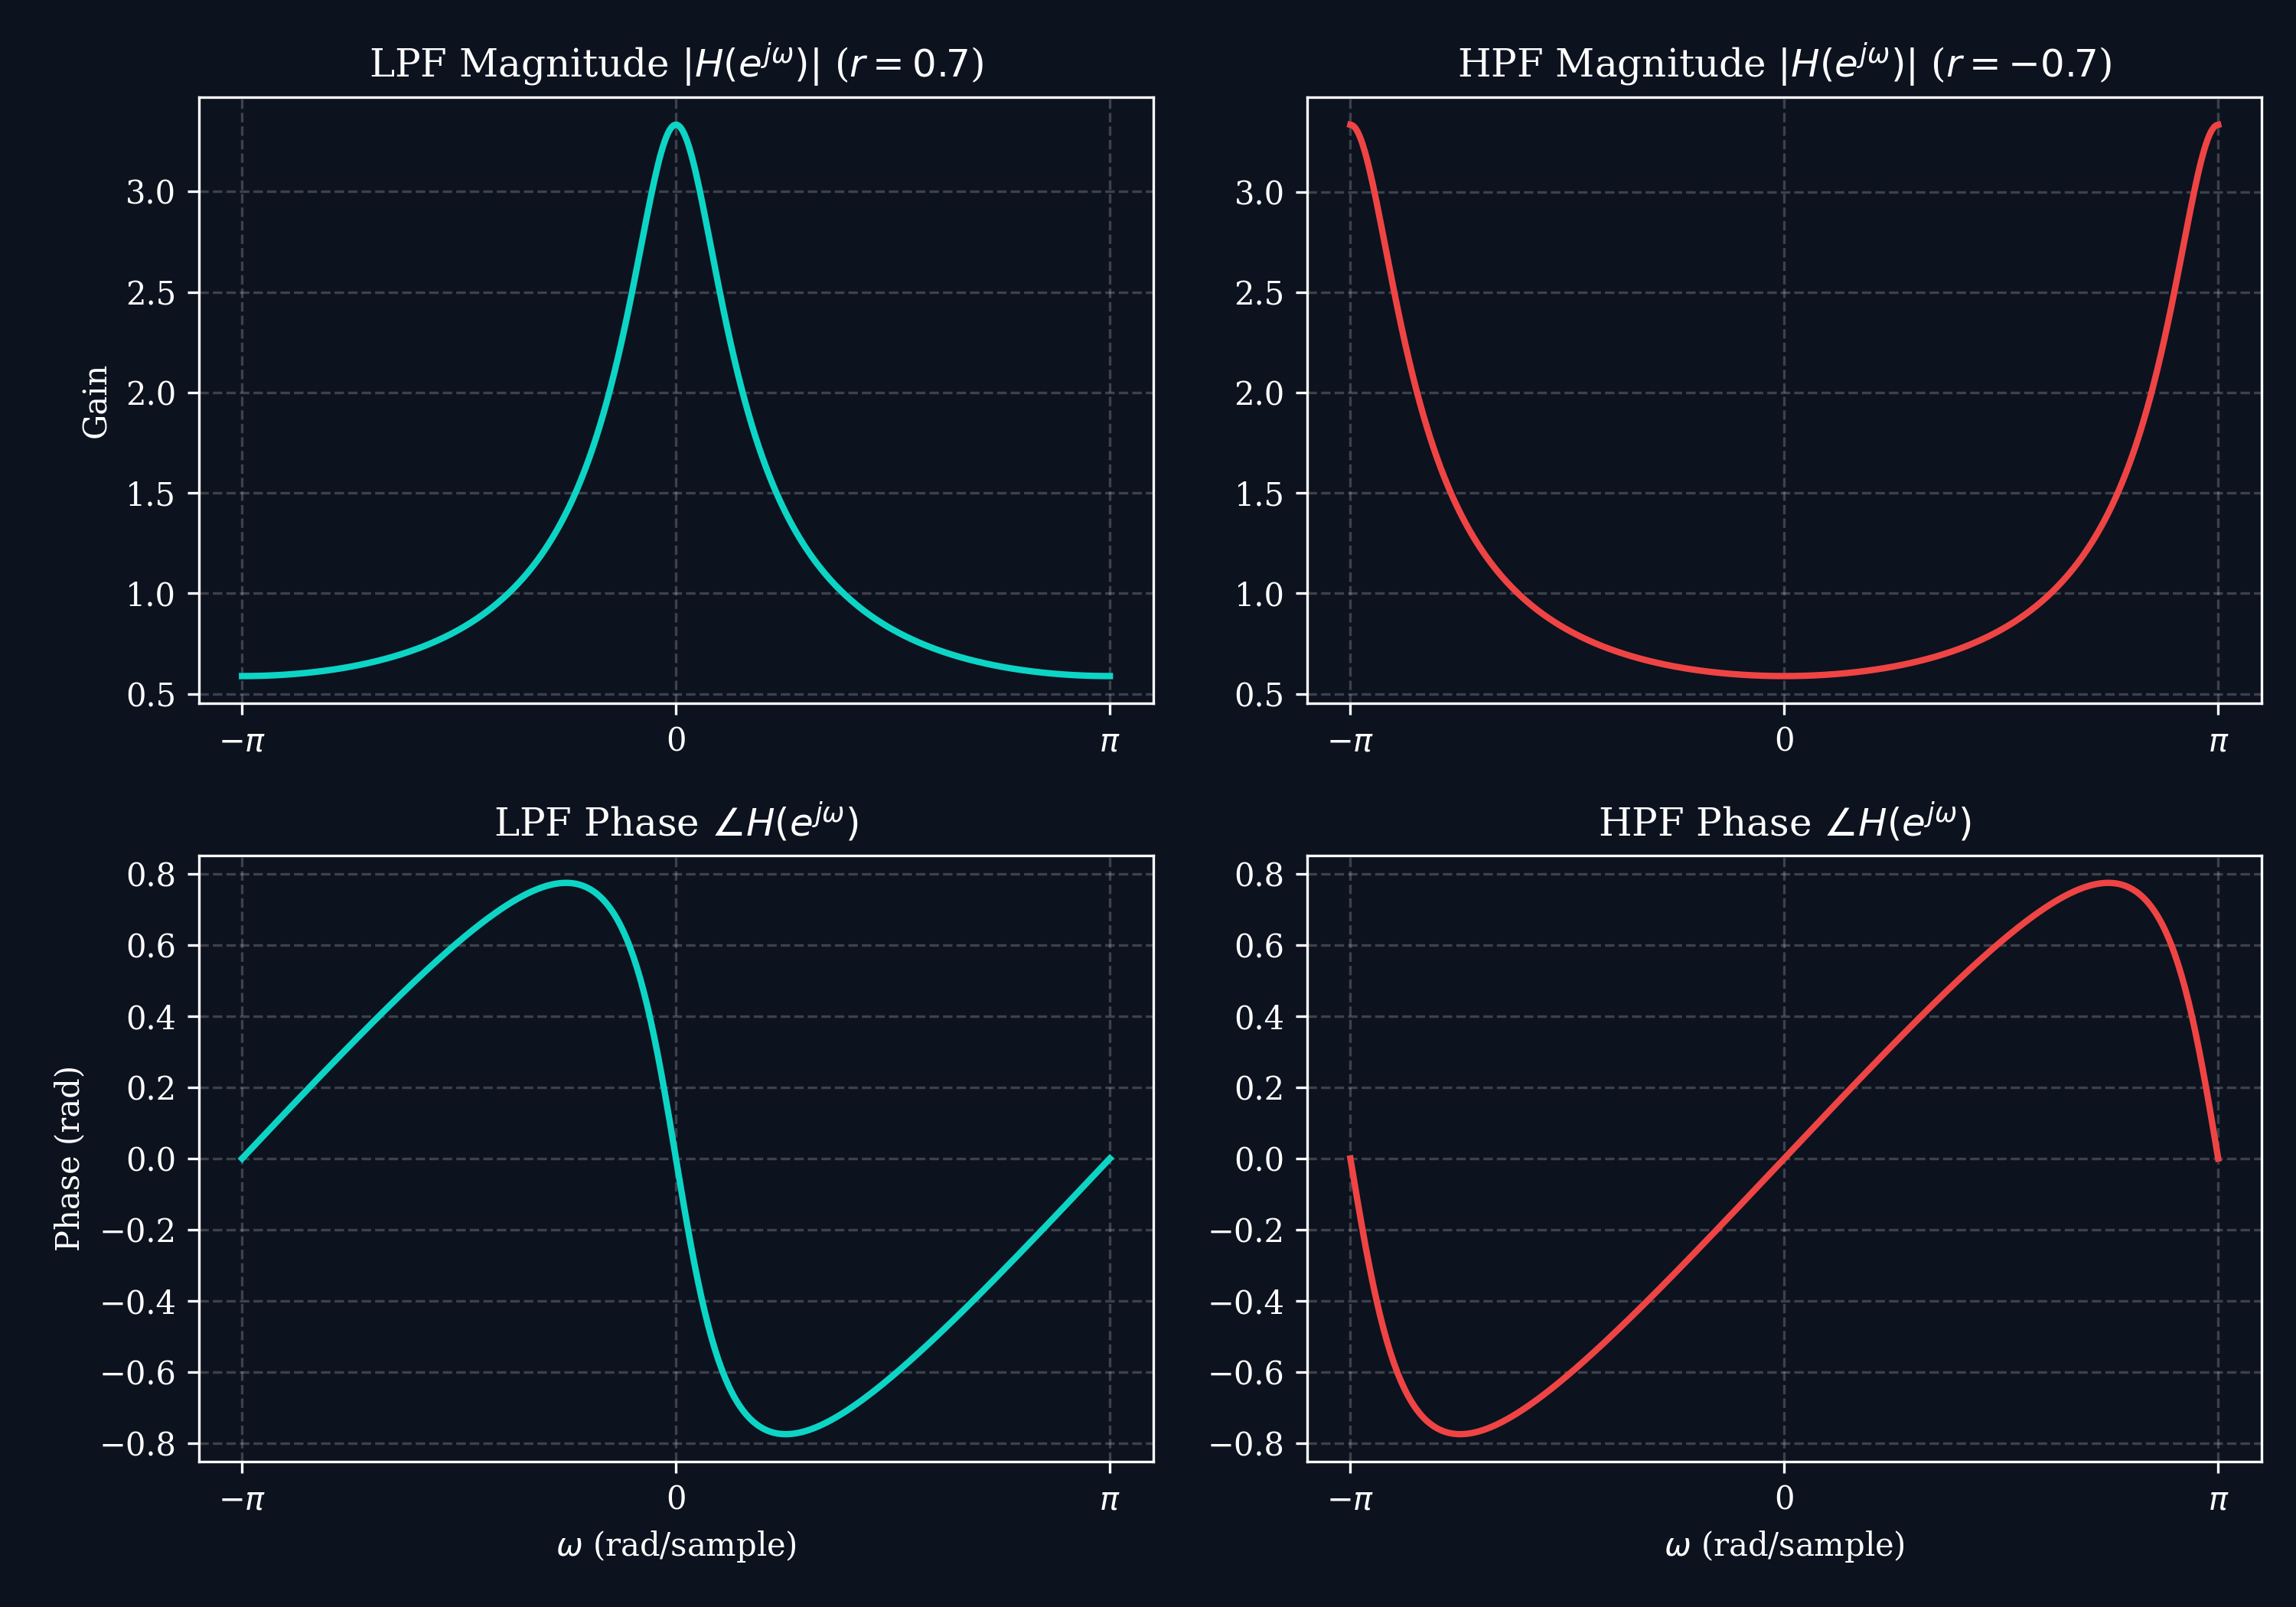
\includegraphics[width=0.85\textwidth]{images/frequency_response_lpf_hpf.png}
\caption{Magnitude and phase responses for first-order digital low-pass and high-pass filters.}
\label{fig:mag_phase_lpf_hpf}
\end{figure}

\section{Phase Delay vs. Group Delay}
\subsection{Mathematical Definitions}
\begin{align}
\text{Phase Delay: } \tau_p(\omega) &= -\frac{\theta(\omega)}{\omega} \\
\text{Group Delay: } \tau_g(\omega) &= -\frac{d\theta(\omega)}{d\omega}
\end{align}

\subsection{Narrowband Envelope Propagation}
Consider a narrowband wave packet input:
\begin{equation}
x[n] = s[n] \cos(\omega_0 n)
\end{equation}
Expanding the phase response $\theta(\omega)$ about $\omega_0$:
\begin{equation}
\theta(\omega) \approx \theta(\omega_0) - \tau_g(\omega_0)(\omega - \omega_0) = -\omega_0 \tau_p(\omega_0) - \tau_g(\omega_0)(\omega - \omega_0)
\end{equation}
The resulting system output is:
\begin{equation}
y[n] \approx |H(e^{j\omega_0})| s[n - \tau_g(\omega_0)] \cos(\omega_0(n - \tau_p(\omega_0)))
\end{equation}
Thus, the envelope $s[n]$ is delayed by the group delay, while the carrier phase is delayed by the phase delay. Figure~\ref{fig:group_delay} compares group delay profiles.

\begin{figure}[H]
\centering
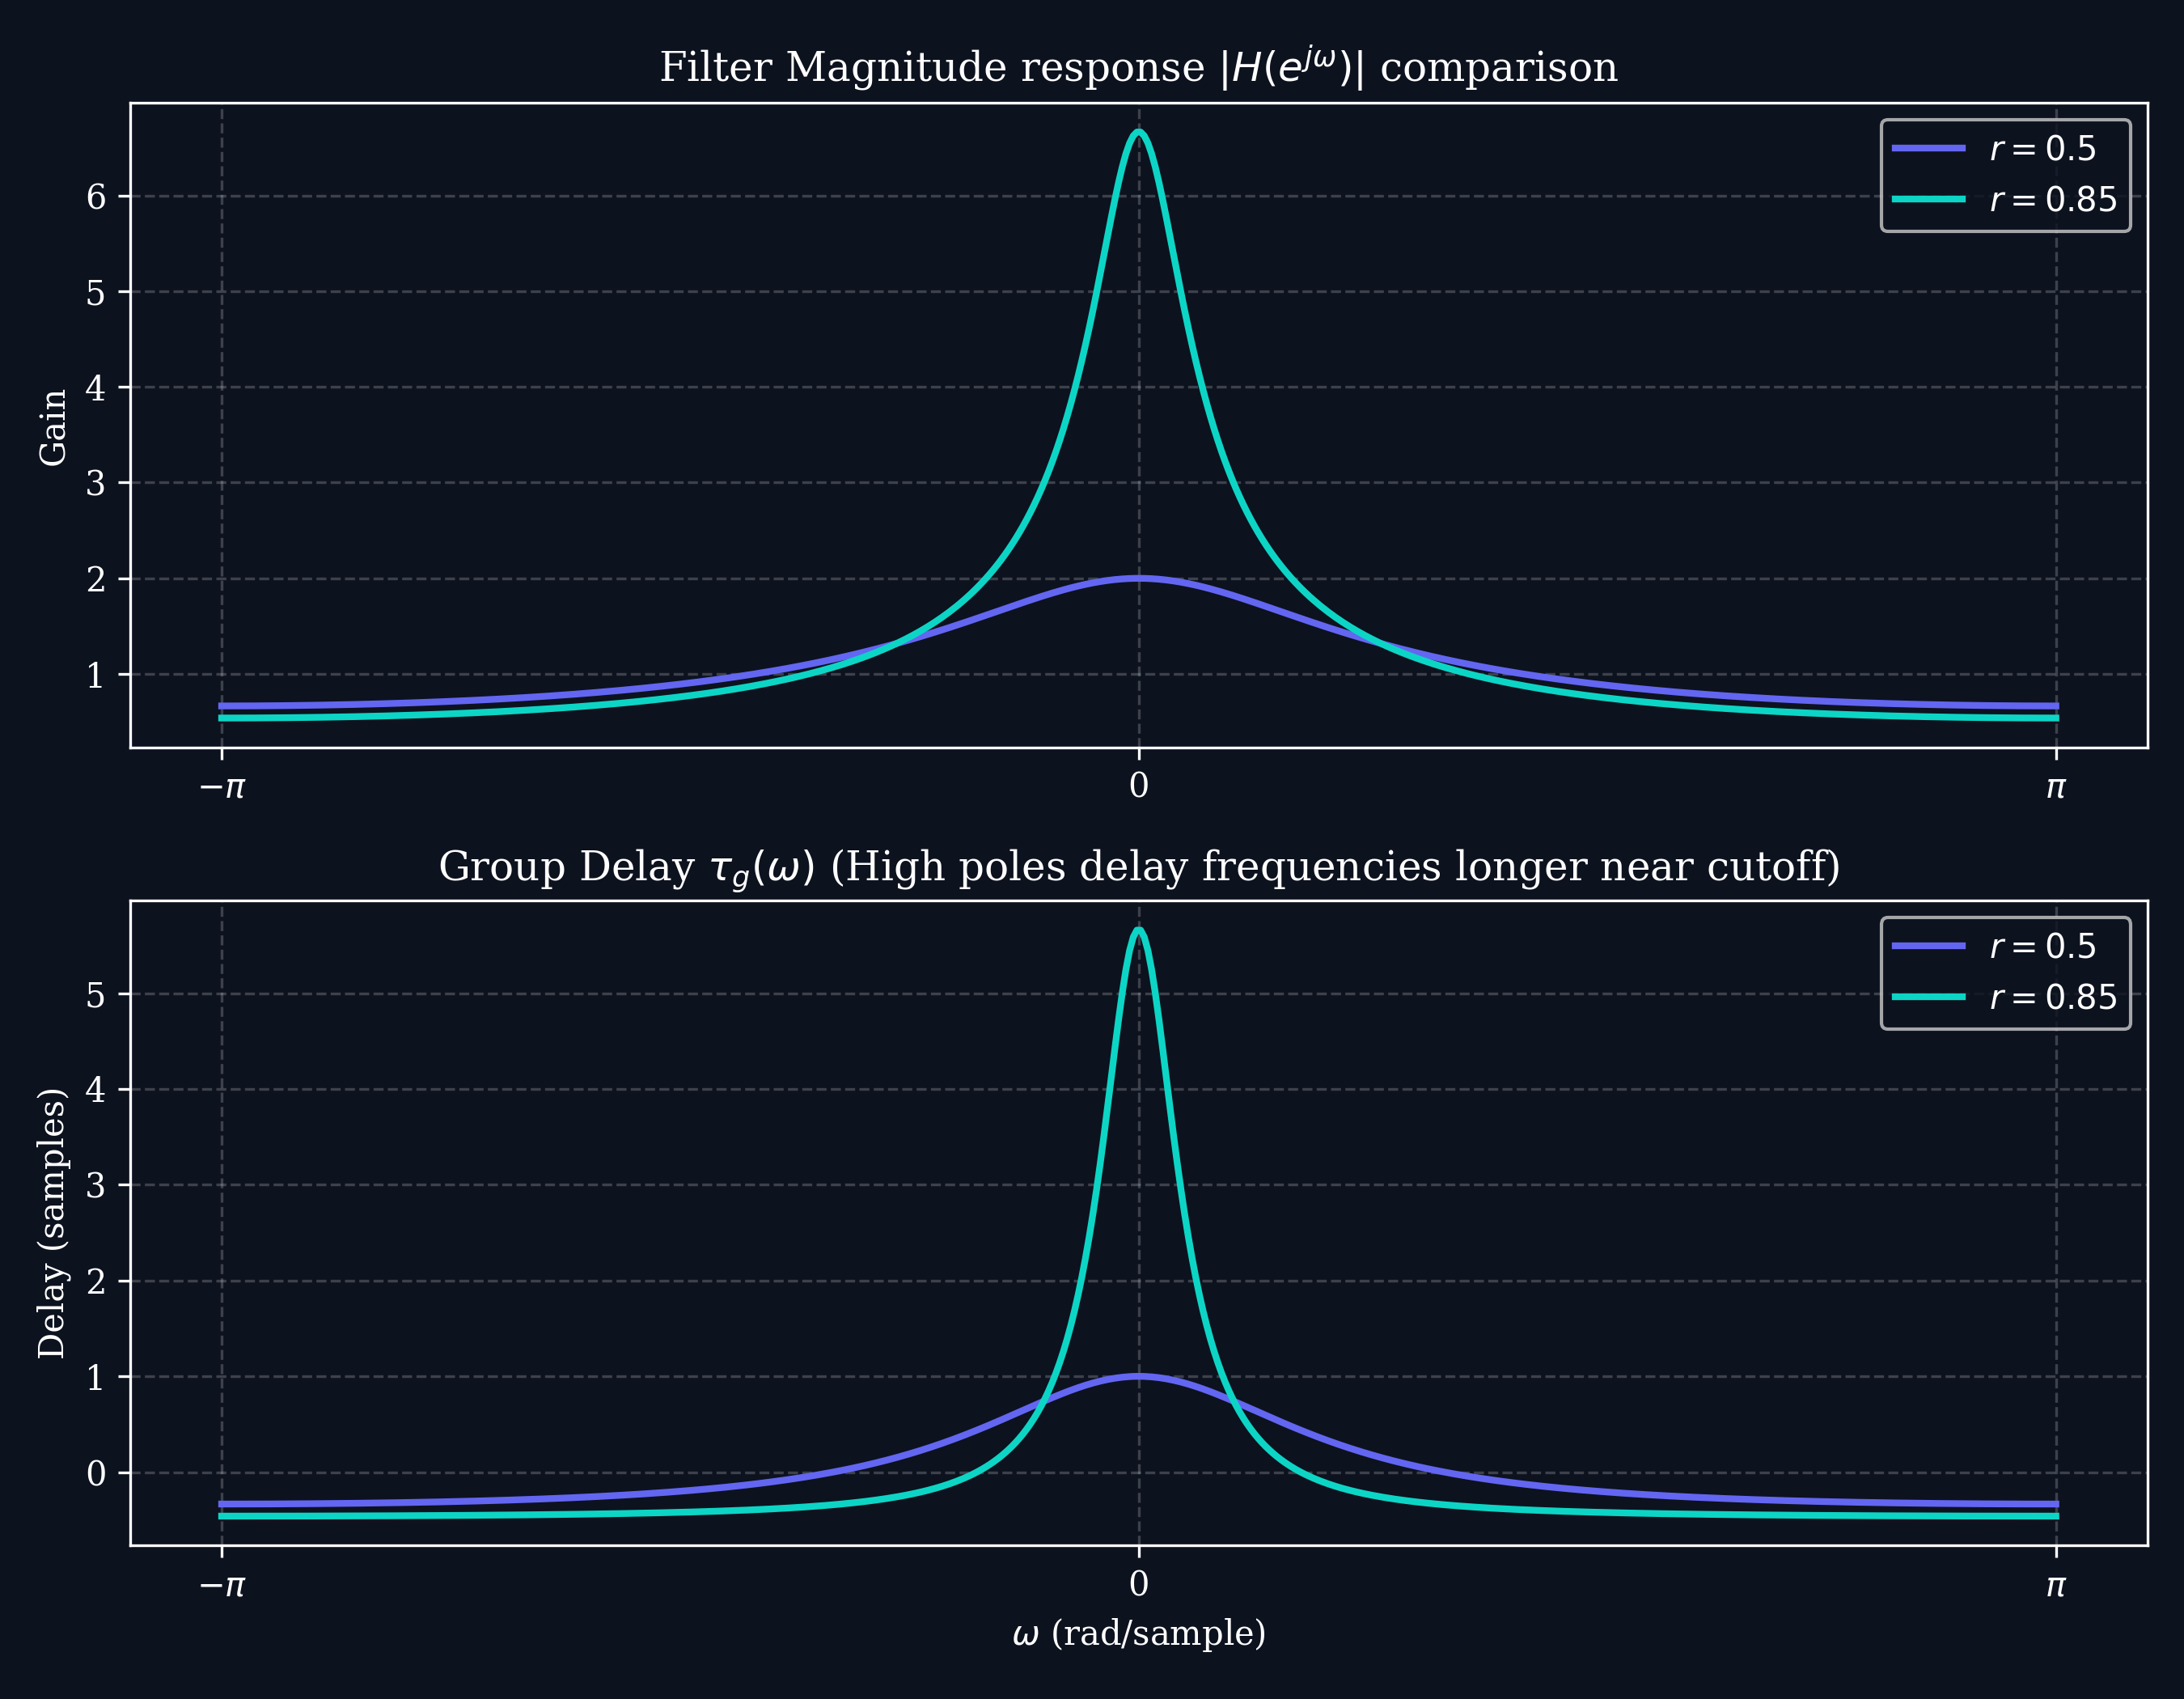
\includegraphics[width=0.85\textwidth]{images/group_delay_analysis.png}
\caption{Filter magnitude and corresponding group delay curves for different pole choices.}
\label{fig:group_delay}
\end{figure}

\section{Group Delay Derivation for First-Order Filter}
Let $y[n] - r y[n-1] = x[n]$ with $|r| < 1$.
\begin{align}
H(e^{j\omega}) &= \frac{1}{1 - r e^{-j\omega}} \\
\theta(\omega) &= -\arctan\left( \frac{r\sin\omega}{1 - r\cos\omega} \right)
\end{align}
Let $u(\omega) = \frac{r\sin\omega}{1 - r\cos\omega}$. Using the derivative of $\arctan(u)$:
\begin{equation}
\frac{du}{d\omega} = \frac{r\cos\omega - r^2}{(1-r\cos\omega)^2} \quad \text{and} \quad 1+u^2 = \frac{1+r^2-2r\cos\omega}{(1-r\cos\omega)^2}
\end{equation}
Combining these terms yields:
\begin{equation}
\frac{d\theta(\omega)}{d\omega} = -\frac{1}{1+u^2} \frac{du}{d\omega} = -\frac{r\cos\omega - r^2}{1 + r^2 - 2r\cos\omega}
\end{equation}
Thus:
\begin{equation}
\tau_g(\omega) = -\frac{d\theta(\omega)}{d\omega} = \frac{r\cos\omega - r^2}{1 + r^2 - 2r\cos\omega}
\end{equation}

\end{document}
